%!TEX root = ../main.tex

\section{아키텍처 개요 및 워크플로}
\label{sec:sdk}

이 섹션에서는 SDK의 개요를 제시합니다.
다양한 사용 시나리오를 지원하도록 구축된 SDK를 사용하면 학술 연구자부터 데이터 과학 실무자에 이르기까지 다양한 배경을 가진 사용자가 프로그래밍 방식으로 고품질 합성 데이터 세트를 생성, 공유 및 조작할 수 있습니다.
툴킷은 명확하게 구조화된 인터페이스를 제공합니다.
허용되는 Apache 버전 2.0 라이센스에 따라 오픈 소스 패키지로 무료로 사용할 수 있습니다.
\verb|pip install -U 'mostlyai[local]'|을 통해 쉽게 설치할 수 있습니다. (Python $\ge 3.10$ 필요)

SDK의 아키텍처는 전용 \emph{품질 보증} 구성 요소와 함께 \emph{커넥터}, \emph{생성기} 및 \emph{합성 데이터 세트}의 세 가지 주요 구성 요소를 중심으로 구성됩니다.
그림~\ref{fig:features}는 이 파이프라인을 보여주며 각 구성 요소와 관련된 주요 기능을 강조합니다.
이러한 아티팩트는 데이터 수집부터 생성 모델 교육 및 공유, 합성 데이터 세트 생성 및 평가까지 사용자를 안내하는 직관적인 워크플로를 형성합니다.
SDK는 로컬 모드와 클라이언트 모드를 모두 지원하지만, 이 작업에서는 둘 다 동일한 기능과 특성을 공유하므로 로컬 모드에만 중점을 둡니다.


\begin{figure*} 
\centering
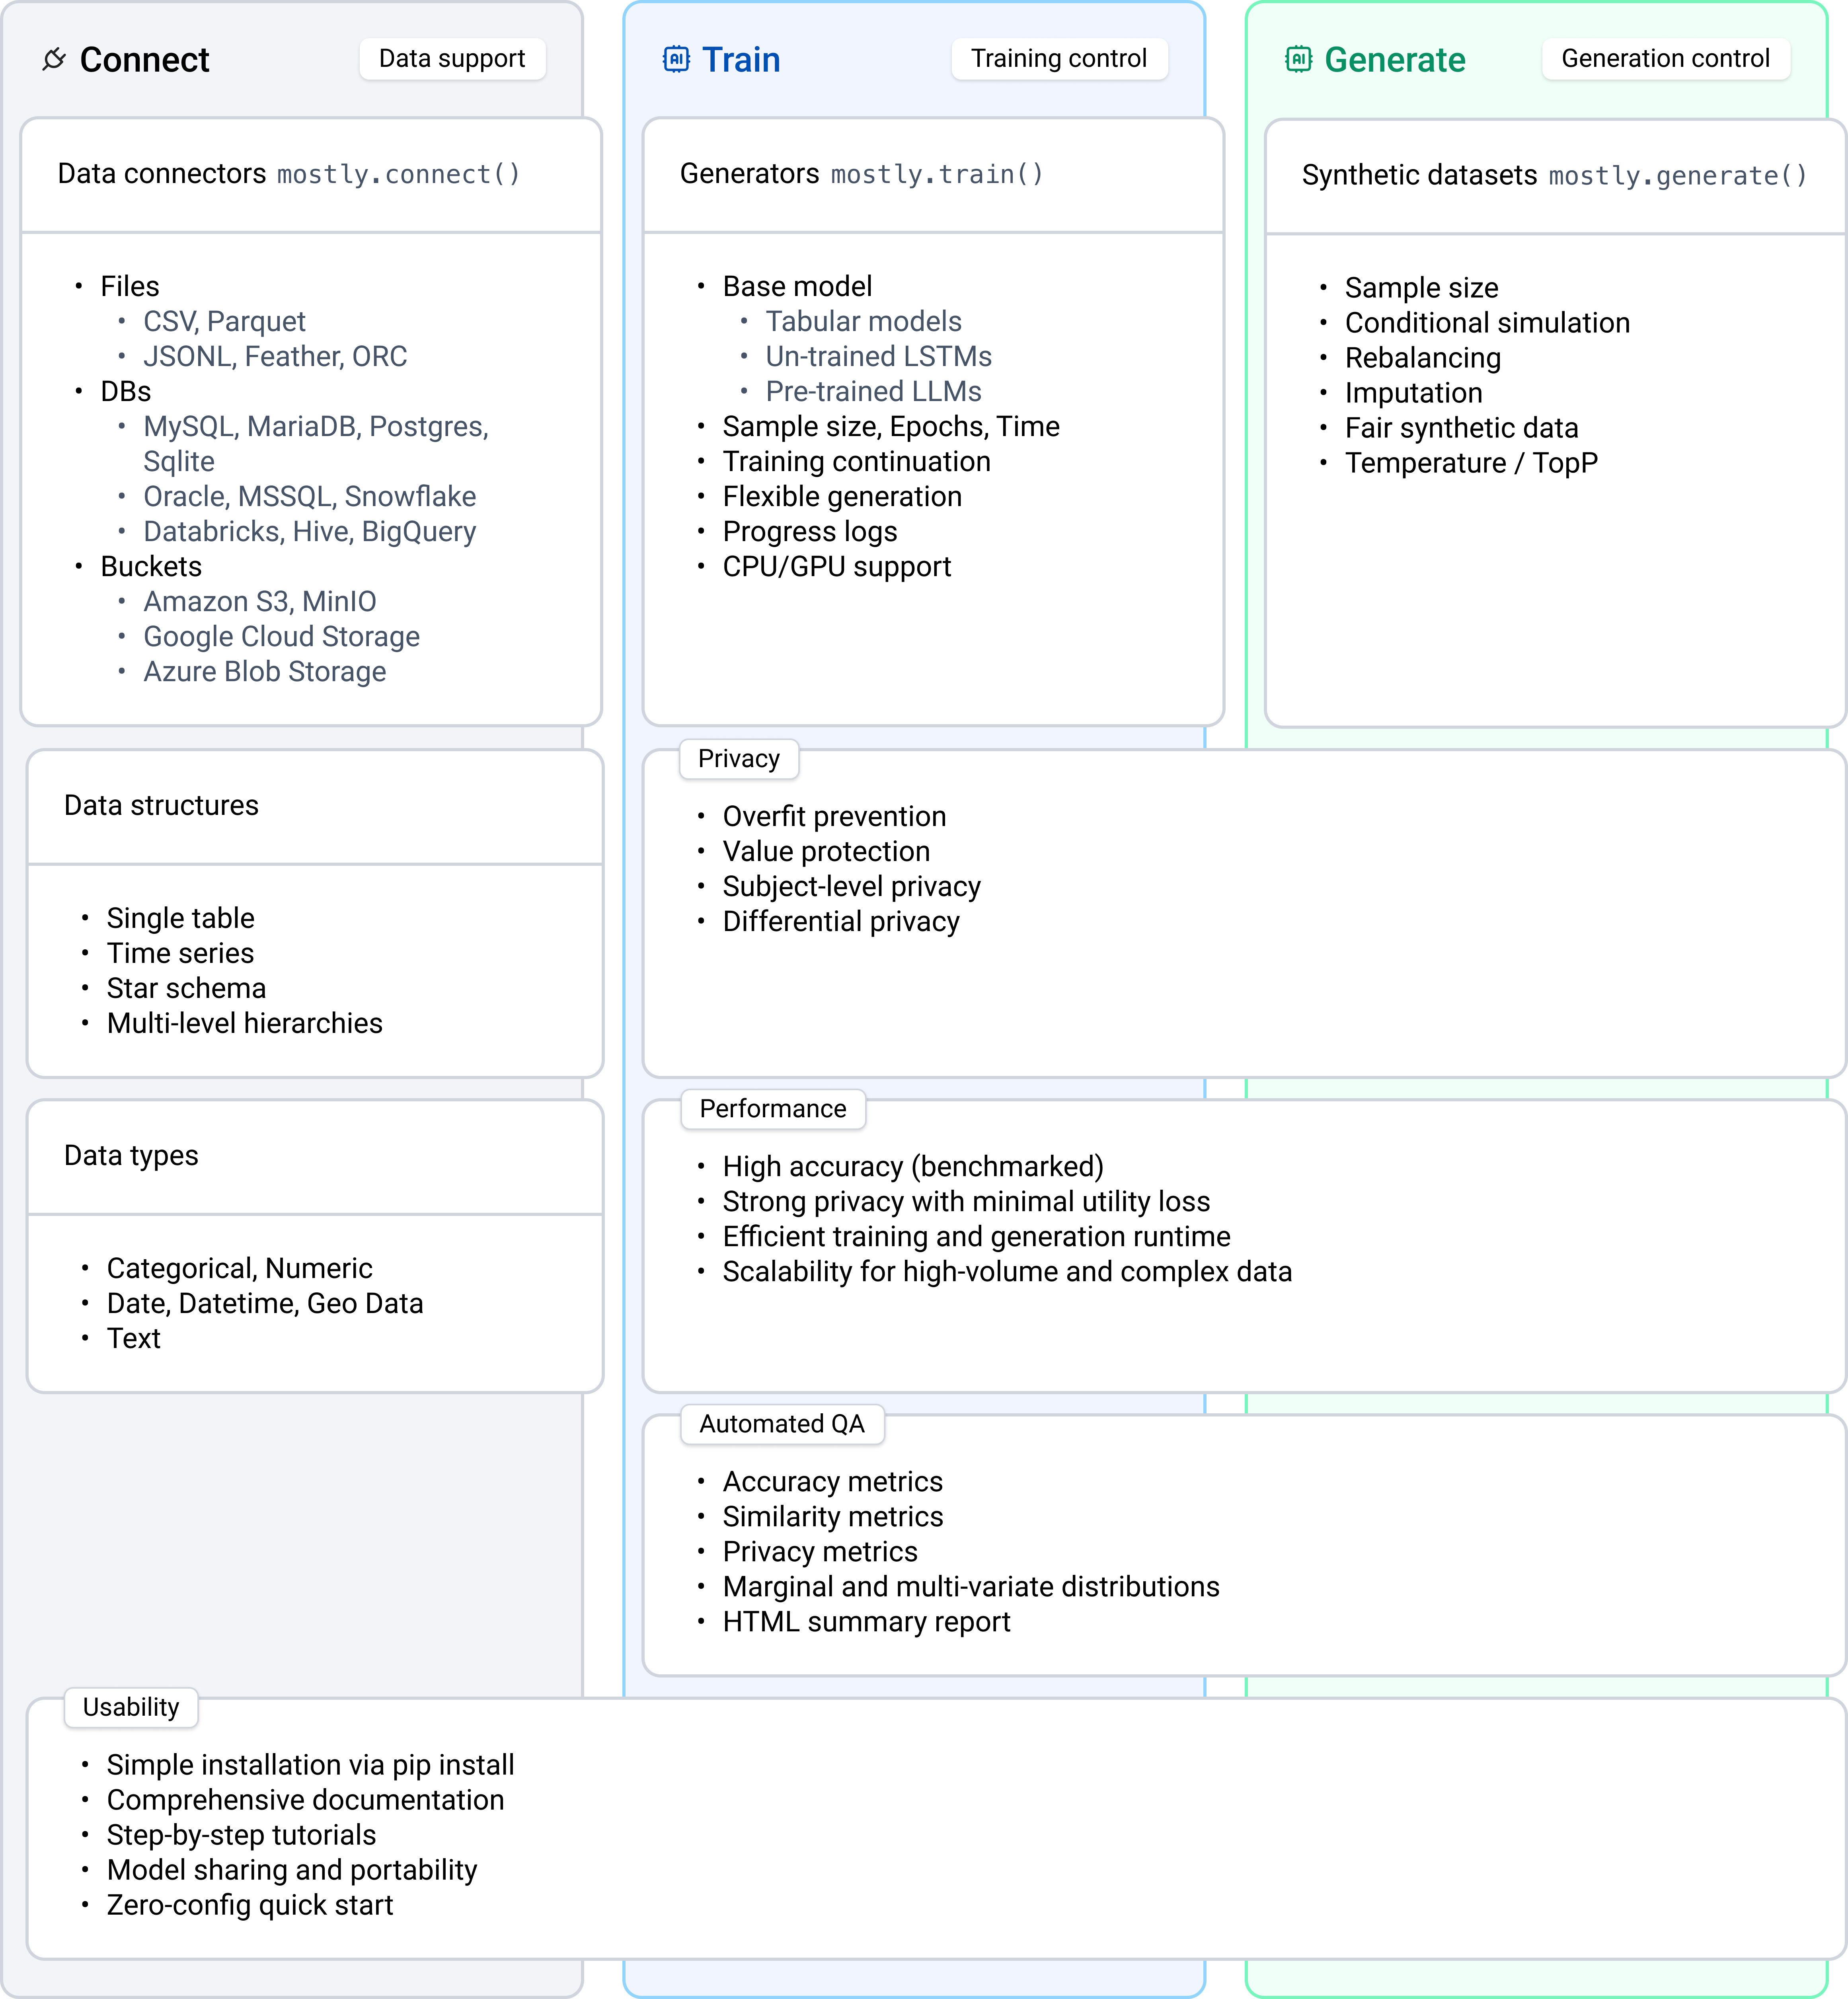
\includegraphics[width=.9\textwidth]{figures/sdk_diagram.png}
\caption{MOSTLY AI 합성 데이터 SDK의 주요 기능 및 기능에 대한 개요입니다. SDK는 \emph{커넥터}, \emph{생성기} 및 \emph{합성 데이터 세트}의 세 가지 주요 아티팩트를 중심으로 구성됩니다. 커넥터는 데이터 수집 및 스키마 정의를 포함한 데이터 지원을 담당합니다. 생성기는 훈련 제어를 처리하며 주로 \texttt{mostly.train()} 기능을 통해 조작됩니다. 생성은 \texttt{mostly.generate()} 함수를 통해 합성 데이터 세트 아티팩트에 의해 제어됩니다. 마지막으로 SDK는 합성 데이터의 안전을 보장하기 위한 개인 정보 보호 메커니즘과 결과 모델 및 데이터 세트의 품질을 평가하기 위한 품질 보증 도구 키트를 통합합니다.}
\label{fig:features}
     % Let's avoid vskip
\end{figure*}


다음에서는 먼저 주요 구성 요소와 품질 보증에 대해 자세히 소개합니다.
그런 다음 SDK의 실제 사용법을 설명하기 위해 간결한 작업 흐름 예제가 제공됩니다.


\subsection{SDK의 핵심 구성요소}
\label{subsec:components}

\paragraph{커넥터}
파이프라인의 첫 번째 단계로 SDK는 다양한 유형의 데이터 소스와 대상을 구성하기 위한 인터페이스를 제공합니다.
이는 훈련 세트를 가져오기 위해 데이터 소스에 액세스하거나 생성된 합성 데이터 세트를 저장할 대상을 지정하는 데 필요한 모든 정보를 캡슐화하는 컨테이너인 \emph{connectors}를 통해 관리됩니다.

커넥터는 널리 사용되는 다양한 데이터베이스 및 클라우드 제공자와의 직접적인 통합을 가능하게 하는 아티팩트입니다.
Figure~\ref{fig:features}에는 SDK가 현재 지원하는 다양한 유형의 커넥터가 나열되어 있습니다.
가장 간단한 수준에서 커넥터는 사용자가 수동으로 업로드한 파일에 대한 로컬 데이터 경로만 지정할 수 있는 반면, 더 복잡한 커넥터에는 키 파일, 비밀번호 및 SSL 인증서와 같은 인증을 위한 자격 증명이 포함될 수 있습니다.

% \begin{table}[t]
% \centering
% \begin{tabularx}{\columnwidth}{l|X}
%     \textbf{Data Source Type} & \textbf{Supported Services} \\
%     \hline
%     Databases & MySQL, PostgreSQL, SQL Server, Oracle, MariaDB, Apache Hive, BigQuery, Snowflake, Databricks \\
%     Cloud Storage & Azure, Google Cloud, AWS \\
%     File Upload & Manual file upload by user.\\
% \end{tabularx}
% \caption{Types of connectors currently supported by our SDK.}
% \label{table:supported_connectors}
% \end{table}

\paragraph{생성기}
교육 데이터를 가져온 후 다음 단계에는 생성 모델을 교육하는 작업이 포함됩니다.
이 단계는 모델 자체의 학습뿐만 아니라 이후에 합성 데이터를 생성하는 데 필요한 데이터 세트에 대한 모든 관련 정보를 캡슐화하는 아티팩트인 \emph{generator}에 의해 처리됩니다.

생성기에는 여러 데이터 유형 지원, 텍스트 모델링을 위한 LLM(대형 언어 모델) 통합, 구성 가능한 교육 설정과 같은 기능이 포함되어 있습니다.
또한 시계열 데이터와 다중 데이터 토폴로지를 처리합니다.
또한 사용자는 추가 개발을 위해 발전기를 가져오고 내보낼 수 있습니다.

\paragraph{합성 데이터세트}
\emph{합성 데이터세트} 구성요소는 훈련된 생성기를 사용하여 합성 데이터를 생성하는 것으로 구성된 파이프라인의 마지막 단계를 처리합니다.
여기에는 데이터 통찰력 및 합성 데이터의 품질 평가를 포함한 여러 추가 아티팩트와 함께 생성된 데이터가 포함됩니다.
또한 재현성을 촉진하기 위해 전체 구성 세부 정보도 제공합니다.
사용자는 레코드를 다시 샘플링하고 다양한 전략으로 데이터를 생성하는 옵션을 사용하여 훈련된 단일 생성기에서 여러 데이터 세트를 생성할 수 있습니다.

\paragraph{합성 데이터 품질 보증 보고서}
SDK는 모든 합성 데이터 생성기에 대해 자동 품질 보증(QA) 보고서를 제공하여 사용자가 생성된 합성 데이터의 충실도와 개인 정보 보호를 모두 평가할 수 있도록 합니다. 각 합성 데이터 생성기에는 포괄적이고 해석 가능한 분석을 위해 표준화된 품질 지표와 대화형 HTML 시각화를 모두 제공하는 상세한 QA 보고서가 함께 제공됩니다.

평가 프레임워크 \cite{qareport}는 홀드아웃 기반 접근 방식을 사용하여 합성 데이터와 원본 데이터를 비교하며 분포 유사성, 임베딩 기반 측정값, 최근접 이웃 거리 등 다양한 정량적 측정항목을 포괄합니다. 순차 및 상황별 기능을 포함하여 다양한 데이터 유형을 지원합니다.

\subsection{기본 작업 재미있는}

SDK는 고품질 합성 데이터에 대한 액세스를 민주화하여 연구자와 실무자에게 힘을 실어줌으로써 광범위한 청중에게 다가가는 것을 목표로 합니다. 이는 사용 편의성, 명확성 및 운영 효율성을 위해 특별히 설계되었습니다.

Figure~\ref{lst:snippet_1}는 합성 데이터 생성을 위한 최소한의 엔드투엔드 워크플로를 보여줍니다. 먼저 SDK가 초기화되고(3행) 예를 들어 Titanic 데이터세트가 \verb|Pandas| DataFrame(라인 5-7). 그런 다음 생성기는 \verb|mostly.train()|을 사용하여 이 데이터에 대해 훈련됩니다. 방법(8-11행). 워크플로는 최종 합성 데이터 세트(13~14행)를 생성하고 액세스하기 전에 QA 보고서(12행)를 표시하여 마무리됩니다.

\begin{figure}%
\begin{lstlisting}[language=Python]
import pandas as pd
from mostlyai.sdk import MostlyAI
mostly = MostlyAI()

original_df = pd.read_csv(
  "https://github.com/mostly-ai/public-demo-data/raw/dev/titanic/titanic.csv"
)
g = mostly.train(
  name="QuickStartDemoTitanic",
  data=original_df,
)
g.reports(display=True)
sd = mostly.generate(g)
df = sd.data()
\end{lstlisting}
\caption{기본적인 작업 예시}%
\label{lst:snippet_1}%
\end{figure}


원본 데이터에 대한 훈련 후 생성기를 내보내고 공유할 수 있으므로 다른 사람들이 원본 데이터를 노출하지 않고도 합성 데이터를 생성하고 생성 설정을 자신의 요구 사항에 맞게 조정할 수 있습니다.
이 기능은 Figure~\ref{lst:snippet_2}에 나와 있습니다.
생성기가 생성되면 고유 ID가 할당됩니다.
특정 생성기에 액세스할 수 있는 권한이 있는 사용자는 1행에 표시된 대로 모델 가중치를 로드할 수 있습니다.
SDK를 사용하면 생성기를 \verb|ZIP|로 가져오고 내보낼 수도 있습니다. 파일은 2행과 3행에 표시된 대로입니다.


\begin{figure}%
\begin{lstlisting}[language=Python]
g = mostly.generators.get('GENERATORID')
path_to_generator = g.export_to_file()
g = mostly.generators.import_from_file(path_to_generator)
\end{lstlisting}
\caption{발전기 공유}%
\label{lst:snippet_2}%
\end{figure}


